%------------------------------------------------------------
%------------------------------------------------------------

\begin{figure*}[!ht]
\centering
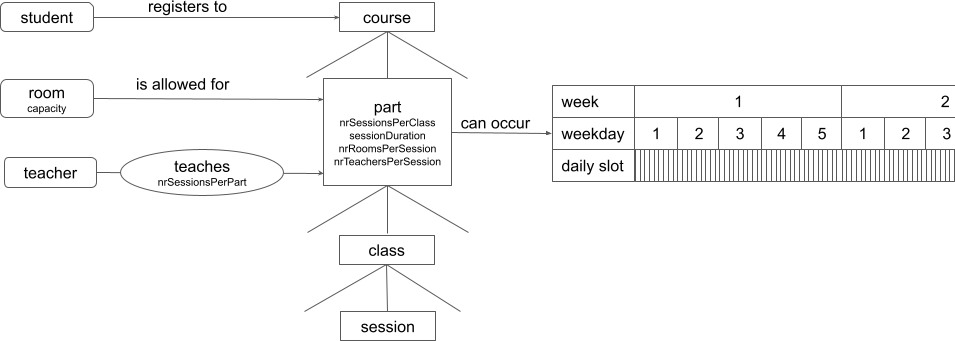
\includegraphics[width=.85\textwidth]{img/utp_entity_model.png}
\caption{Entity model}
\label{fig:utp-entity-model}
\end{figure*}

\subsection{Entity model}
\label{sec:entity-model}
The entity model of a {\UTP} instance defines its schedule horizon, course structure and resources, as well as the properties of entities and the relational maps (see Figure~\ref{fig:utp-entity-model}).  
First, the model uses a time grid that decomposes into weeks, weekdays and daily slots, % (see Figure~\ref{fig:utp-time-grid}),
the number of which is instance-specific.
Weeks share the same weekdays and weekdays the same daily slots.
The latter make up 24 hours and have the same duration (e.g. 24 daily slots will represent 1 hour each, 1440 daily slots represent 1 minute each).
%\marc{C'est pas forcément mesuré en minutes ... Dans nos exemples oui, mais justement c'est custom.
%Il faudrait dire "The latter makes up 24 hours and have the same duration, meaning that 3 dailyslots will represent 8 hours each, or 1440 dailyslots represent 1 minute each." ?}
Note that neither successive weeks nor successive weekdays are assumed to be consecutive.
The schedule horizon is implicitly defined by the series of time slots mapping to week, weekday and daily slot combinations.
Slots hence serve as time points to represent start and end times of course sessions and to measure durations (session length, travel times).

% % For one-column wide figures use
% \begin{figure}[h]
% % \includegraphics{utp-time-grid.eps}
% \caption{{\UTP} 3-layered time grid}
% \label{fig:utp-time-grid}
% \end{figure}

Courses have a tree-structure wherein each course (i.e., course topics) decomposes into parts (lecture, practical work \ldots), parts into classes, and classes into sessions.
Class sessions are the elementary tasks to schedule when solving a {\UTP} instance
and the model fixes their number, duration and sequencing.
On the one hand, the classes of a course part are decomposed into an identical number of sessions of equal duration, both constants being part-specific.
Although this approach forbids alternative class decompositions using variable session durations, 
it %provides flexibility for handling sessions independently wrt. scheduling and resource allocation.
%Fixed decompositions also 
facilitates the formulation of requirements which depend on clear-cut sessions (e.g., planning parallel sessions ``mid-way'' through a course).
On the other hand, the model requires that the sessions of a class be ranked and sequenced accordingly in any solution.
Note that sessions are considered uninterruptible and, in particular, may not overlap two days. 

{\UTP} resources fall into 3 types, namely, rooms, teachers, students (gathered into groups).
All the resources of an instance are declared and typed in the entity model.
In practice, various restrictions resulting from upstream processes apply on the resourcing and timing of courses.
Basic restrictions come in the form of compatibility constraints that list the suitable rooms, eligible teachers, candidate students and allowed times for the different courses 
(e.g., faculties prescribing degree-specific time grids, departments implementing room pooling policies, %alternative 
teachers applying for courses, student registrations). %registering to courses).
Such constraints are built in the entity model but scoped differently depending on resource types.
Specifically, each course part is assigned sets of possible start times, rooms and teachers which propagate automatically to all its sessions.
As for students, course registrations are listed separately and %the possible students for a session are those registered to the course it sits in.
any student registered to a course is considered a possible candidate for each of its sessions.

Beyond plain compatibility, resource utilization is subject to demand and capacity constraints.
Since modalities differ from one environment to the next, the language supports both disjunctive and cumulative resources as well single- and multi-resource sessions. 
Students, teachers or rooms qualify as cumulative resources if they 
can attend, teach or host simultaneous sessions. %, respectively.
Cumulative resources are paramount to meet flexible attendance requirements (e.g., students assigned optional tutoring sessions that may overlap with mandatory courses) or to handle multi-class events (e.g., rooms hosting joint exam or conference sessions).
The schema assumes no limit on the number of parallel sessions teachers and students may attend.
Rooms however may only host class sessions whose cumulated headcount
is within their capacity.
Upper bounds on room capacity and class size are encoded for all rooms and classes in the entity model with the possibility to leave room capacity unbounded (e.g., virtual rooms). 
Note that all resources default to cumulative resources but this assumption may be overridden using disjunctive rules on a per resource basis.
% a {\UTP} instance may freely mix disjunctive and cumulative resources. 

A multi-resource session is a session requiring multiple resources of the same type. %at any point in time.
The need for sessions using multiple rooms or teachers arises in many practical situations (e.g., multi-room sessions for hybrid teaching, joint supervision of practical work sessions, exams requiring several adjudicators).
The number of resources required per session is typically fixed on course parts and  
such restrictions are expressed in the entity model through cardinality constraints. %that are lifted to course parts. 
Specifically, each course part indicates the number of teachers required per session 
and whether its sessions are single- or multi-rooms.
Multi-room sessions impose specific constraints:
allocated rooms are disjunctive for the time of the session only and their total capacity is considered for hosting the students attending the session.
Note that the model allows for sessions without teachers or rooms (e.g., unsupervised student projects). 
%a {\UTP} instance may freely mix single- and multi-resource sessions as well as disjunctive and cumulative resources. 

The entity model also encodes flow constraints that govern the distribution of students and teachers over courses. 
These constraints %relating to the distribution of students and teachers over courses 
are usually elicited ahead of scheduling during registration and capacity planning stages (e.g., departments distributing session volumes among designated teachers). 
As mentioned above, students only register for courses, not for classes nor sessions, and solving a {\UTP} instance involves determining student-to-class assignments that are consistent with the course structure.
Specifically, every student must be assigned a single class in each part of a course he has registered to and must attend all sessions of these classes. 
Group nesting constraints may also be stated between classes %. %to enforce equality or set inclusion relations between their sets of participants.
%These constraints serve 
to implement course-specific or cross-course sectioning policies (e.g., aggregating student groups bottom-up from practicals to lectures, enforcing identical groups between classes of different courses of a curriculum).
As for staff distribution, each teacher is assigned a fixed volume of sessions in each course part he is eligible for, leaving teacher-to-session assignment decisions to solvers.

Note finally that the language provides the ability to label entities and define custom classes of elements (e.g., teams of teachers, blocks of rooms). %that complement the built-in types. 
%Entities sharing the same label form a type of their own named after the label.
Labels complement built-in types and entity identifiers as a means to select entities within rules.
  


%Rules may then help to enforce instance-specific scheduling or resource allocation constraints on any entity or group of entities, e.g. casting a problem instance as a pure disjunctive scheduling problem.

%First, teachers are explicitly represented on par with rooms. Student groups may optionally be modelled too to cater for workflows where student sectioning is performed ahead of session scheduling. 

%The {\UTP} schema also differs on the way sessions are time-framed in a class. Indeed a class' sessions are just chronologically ranked and specific scheduling requirements are enforced per class (e.g., periodicity) or across classes (e.g., simultaneity) through explicit rules.
%while leaving the opportunity to jointly state and solve both problems. Second, it represents teachers explicitly, allows for class sessions requiring multiple resources (e.g., multi-room or -teacher sessions),
%and supports resource distribution constraints (e.g., eligible teachers and their workload per course part measured in sessions).
%and rooms %(including virtual rooms) 


We formalize below the entity model and introduce notations that will be used thereafter.
Let ${\ENTITY}$ denote the set of entities
and ${\SESSION}$ the set of sessions.
${\ENTITY}$ is partitioned into   
a set of courses ${\COURSE}$, 
a set of course parts ${\PART}$, 
a set of classes ${\CLASS}$, 
a set of students ${\STUDENT}$, 
a set of teachers ${\TEACHER}$,
a set of rooms ${\ROOM}$,
and the singleton domain of courses ${\COURSES}$ 
(${\COURSES}=\myset{\COURSE}$). 
Let 
%${\COURSES}$ denote the course domain, 
%${\COURSE}$ the set of courses (${\COURSES}=\myset{\COURSE}$), 
%${\PART}$ the set of course parts, 
%${\CLASS}$ the set of classes, 
%${\SESSION}$ the set of sessions, 
%${\STUDENT}$ the set of students, 
%${\TEACHER}$ the set of teachers, 
%and 
%${\ROOM}$ the set of rooms.
$
{\TYPE}
=
\myset{
{\COURSES}, 
{\COURSE},
{\PART},
{\CLASS},
{\STUDENT},
{\TEACHER},
{\ROOM}
}
$
denote the set of entity types
(${\ENTITY}=\setunion{X}{\TYPE}{X}$)
and 
$
{\prec}
=
\myset{
({\COURSES},{\COURSE}),
({\COURSE},{\PART}),
({\PART},{\CLASS}),
({\CLASS},{\SESSION}),
({\STUDENT},{\COURSE}),
({\TEACHER},{\PART}),
({\ROOM},{\PART})
}
$
denote the relation over 
${\TYPE}\cup\myset{\SESSION}$ 
that models the course hierarchy
and the distribution of resource types over course components.
${\prec^{*}}$
%${\preceq^{*}}$
denotes the transitive %and reflexive 
closure of
${\prec}$ 
over
${\TYPE}\cup\myset{\SESSION}$
and
${\maptype{X}{Y}}:X\rightarrow2^{Y}$
denotes the function mapping each element of $X$ to its set of compatible elements in $Y$
for each pair %$(X,Y)$ such that 
%$X{\preceq^{*}}Y$.
$X{\prec^{*}}Y$.
For instance, 
${\maptype{\STUDENT}{\COURSE}}$ 
represents the distribution of students over courses, 
${\maptype{\COURSE}{\PART}}$ 
the decomposition of courses into course parts,
and ${\maptype{\STUDENT}{\PART}}$ 
the inferred distribution of students over course parts.
The functions corresponding to the pairs of $\prec$
are directly encoded in the entity model
and the remaining functions are defined inductively using recursive aggregation. 
Rule (\ref{model:hierarchy}) below models the hierarchical decomposition of course elements\footnote{$\sqcup$ denotes the disjoint union operation, i.e. set union over pairwise disjoint sets.}
and
Rule (\ref{model:transitivity}) is the closure rule over 
%$\preceq^{*}$. 
$\prec^{*}$. 
%Rule (\ref{model:symmetry}) enforces symmetry over all compatible pairs,
%and Rule (\ref{model:selfmap}) completes the model with self-maps. 

%\todo[inline]{i en indice dans les équations suivantes, formulation non expliquée. $d_i$ serait l'ensemble des couples (a,b) de la relation tels que a=i ?}
%\vincent{Dans ce cas, comme d est une fonction, ça serait plutôt $d^{Y,Z}(i)$}
%\marc{On en discutait avec DG et effectivement c'est ce qu'on a conclu. Cependant, plus tard cette notation est réutilisée avec en indice des ensembles de valeurs. Il faut donc faire attention à bien introduire cette notation.
%De plus je rajouterais une petite remarque : $\forall (X,Y)$ et non $\forall X,Y$ ?}

\begin{multline}
\forall (X,Y) \in  \myset{ ({\COURSES},{\COURSE}), ({\COURSE},{\PART}), ({\PART},{\CLASS}), ({\CLASS},{\SESSION}) }: \\
Y=\setpartition{i}{X}{\map{X}{Y}{i}} \label{model:hierarchy}
\end{multline}
\begin{multline}
\forall X,Y,Z \in {\TYPE}\cup\myset{\SESSION}:\\
\mbox{\hspace{-10em}}X\preceq^{*} Y\preceq^{*} Z 
\Rightarrow \\
(\forall i \in X:
\map{X}{Z}{i}=\setpartition{j}{\map{X}{Y}{i}}{\map{Y}{Z}{j}}
 \label{model:transitivity})
%%
%%\forall X,Y \in {\TYPE}:
%%X\preceq^{*} Y 
%%\Rightarrow 
%%(\forall i \in X, j \in Y:
%%j \in \domarg{X}{Y}{i} \Leftrightarrow i \in \domarg{Y}{X}{j}
%%) \label{model:symmetry}\\
%%
%\forall X \in {\TYPE}\cup\myset{\SESSION},
%i \in X:
%\domarg{X}{X}{i} = \myset{i} \label{model:selfmap}
%%
\end{multline}

%We shall denote by
%${\RANK}$
%the range of session ranks,
%${\maptype{\RANK}{\SESSION}}:\RANK\rightarrow2{^\SESSION}$
%the rank-based partitioning of sessions,
%and
%${\LABEL}$
%the set of labels 
%(${\LABEL}\subseteq2^{{\ENTITY}}$)
%completed 
%with the whole set of entities %to mock label optionality
%($\ENTITY\in{\LABEL}$)
%and singleton entities %to support identity-based selection
%($\myset{\myset{e}\ |\ e\in{\ENTITY}}\subseteq{\LABEL}$).
%As discussed in section~\ref{sec:rules},
%labels are optional filters used in rules to select entities
%hence the formal inclusion of $\ENTITY$ in ${\LABEL}$ to mock label optionality.
%Likewise, entity identifiers are used as an alternative to labels
%hence the inclusion of singleton entities in ${\LABEL}$.
